\chapter{Un réseau de neurones auto-organisé : les cartes de kohonen}
\graphicspath{{02-SOM/}}
// Kohonen : il faut surprendre encore ! Par quel 
bout le prendre ? 
→ Appuyer sur les cartes 1D
→ Comment ca se fait qu’on les utilise pas de ouf ? 
→  Intérêt de la topologie de la carte. Dans une carte seule, est ce que c’est vraiment utile ?
→ Questionnement informatique : qu’est ce qui se passe en fait dedans, mais c’est quand même rigolo.

\section{Principe Général}
Une carte de Kohonen est un graphe dans lequel chaque noeud possède un poids $\omega$ appartenant à l'espace des entrées. L'algorithme repose ensuite sur l'adaptation de ces poids, en prenant en compte les connexions dans le graphe, afin de représenter les données d'entrées. 
Ainsi, n'importe quel graphe pourrait être considéré; le plus souvent, une grille 2D est utilisée.

\section{Approche topologique des cartes de Kohonen}

La notion de voisinage et de topologie est un élément clé des cartes de Kohonen. Le voisinage est en effet pris en compte lors de l'apprentissage et lors de l'interpretation des cartes. Cependant, ce voisinage est généralement défini, dans les applications des cartes, comme un bonus par rapport aux KMeans, une aide à la convergence et à la vitesse de dépliement. Pourtant c'est la l'essence même d'une carte de Kohonen: projeter des éléments sur un graphe, ce qui nous permet de faire des calculs sur des positions plutot que des données de grandes dimensions. 
\begin{figure}
\centering
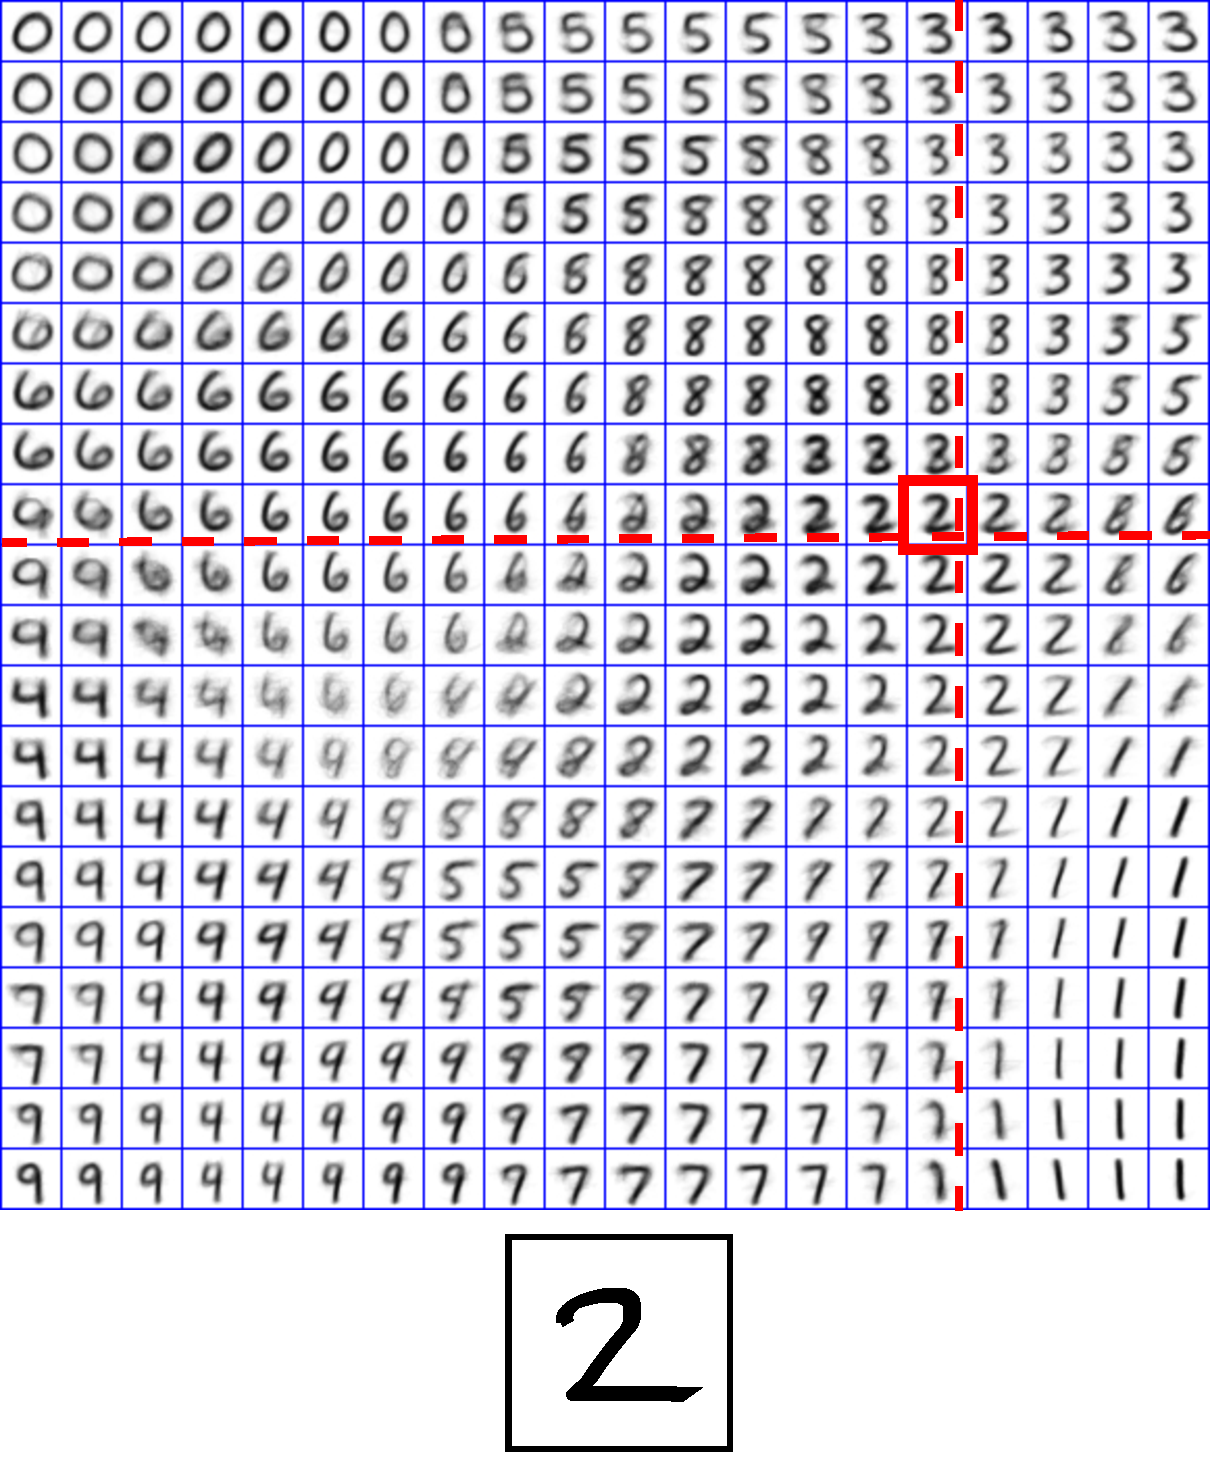
\includegraphics[width=\textwidth]{digits002.pdf}
\caption{Une carte de Kohonen s'organise en zones dont les poids sont proches dans l'espace des entrées. Chaque entrée présentée à la carte peut alors être représentée par la valeur de la position du BMU correspondant dans la carte. Les entrées sont projetées sur le carré $[0,1] \times [0,1]$.}
\end{figure}

\section{Principes d'organisation}


\section{Travaux préliminaires sur les architectures de cartes de Kohonen}



\section{A trier}
De la biologie a la computation : patterns temporels des neurones impulsionnels vs SOM. 